% !BIB program = bibtex
% !TeX root = ../main.tex

\chapter{Problem Formulation}

\section{Problem Description}

The object of this research is to minimize the maximum percentage of cost saving when a passenger chooses to carpool, with consideration of the number of drivers, car capacity and routing limit constraints.

Take Figure 3-1 as an example scenario; Passenger 1 and Passenger 2 are requesting a trip. When Passenger 1 chooses to take a ride by himself/herself, called "exclusive" riding shown as Figure 3-2, it would cost \$5. We can describe the scenario as a shortest path problem from $S$ to $D_1$, and $P_1$ is a must-pass node. We use Steiner tree to solve this kind of shortest path problem with must-pass nodes. Passenger 2's "exclusive" riding would also cost \$5 in Figure 3-3. In this case, it would be a shortest path problem from $S$ to $D_2$ with $P_2$ as a must-pass node.

When the passengers choose to take a carpool, which is called "sharing" riding. We can describe the scenario as a shortest problem from $S$ to $D_1$ with $P_1$, $P_2$ and $D_2$ as must-pass nodes or $S$ to $D_2$ with $P_1$, $P_2$ and $D_1$ as must-pass nodes. In Figure 3-4 is one of the best case, which would cost \$8 for all the passengers, in Figure 3-5 would cost the same \$8 and both of the fares they could share are \$5 ( $\overline{P_2D_1}$ and $\overline{P_2D_2}$ respectively); however, in Figure 3-4 would cost $\overset{\overline{P_1P_2}}{1} + \frac{1}{2} \times \overset{\overline{P_2D_1}}{5} = \$3.5$ for Passenger 1 and $\frac{1}{2} \times \overset{\overline{P_2D_1}}{5} + \overset{\overline{D_1D_2}}{1} = \$3.5$ for Passenger 2, in Figure 3-5 would cost $\overset{\overline{P_1P_2}}{1} + \frac{1}{2} \times \overset{\overline{P_2D_2}}{5} + \overset{\overline{D_2D_1}}{1} = \$4.5$ for Passenger 1 and $\frac{1}{2} \times \overset{\overline{P_2D_2}}{5} = \$2.5$ for Passenger 2.

\begin{figure}[htp]
  \centering
  \captionsetup{justification=centering}
  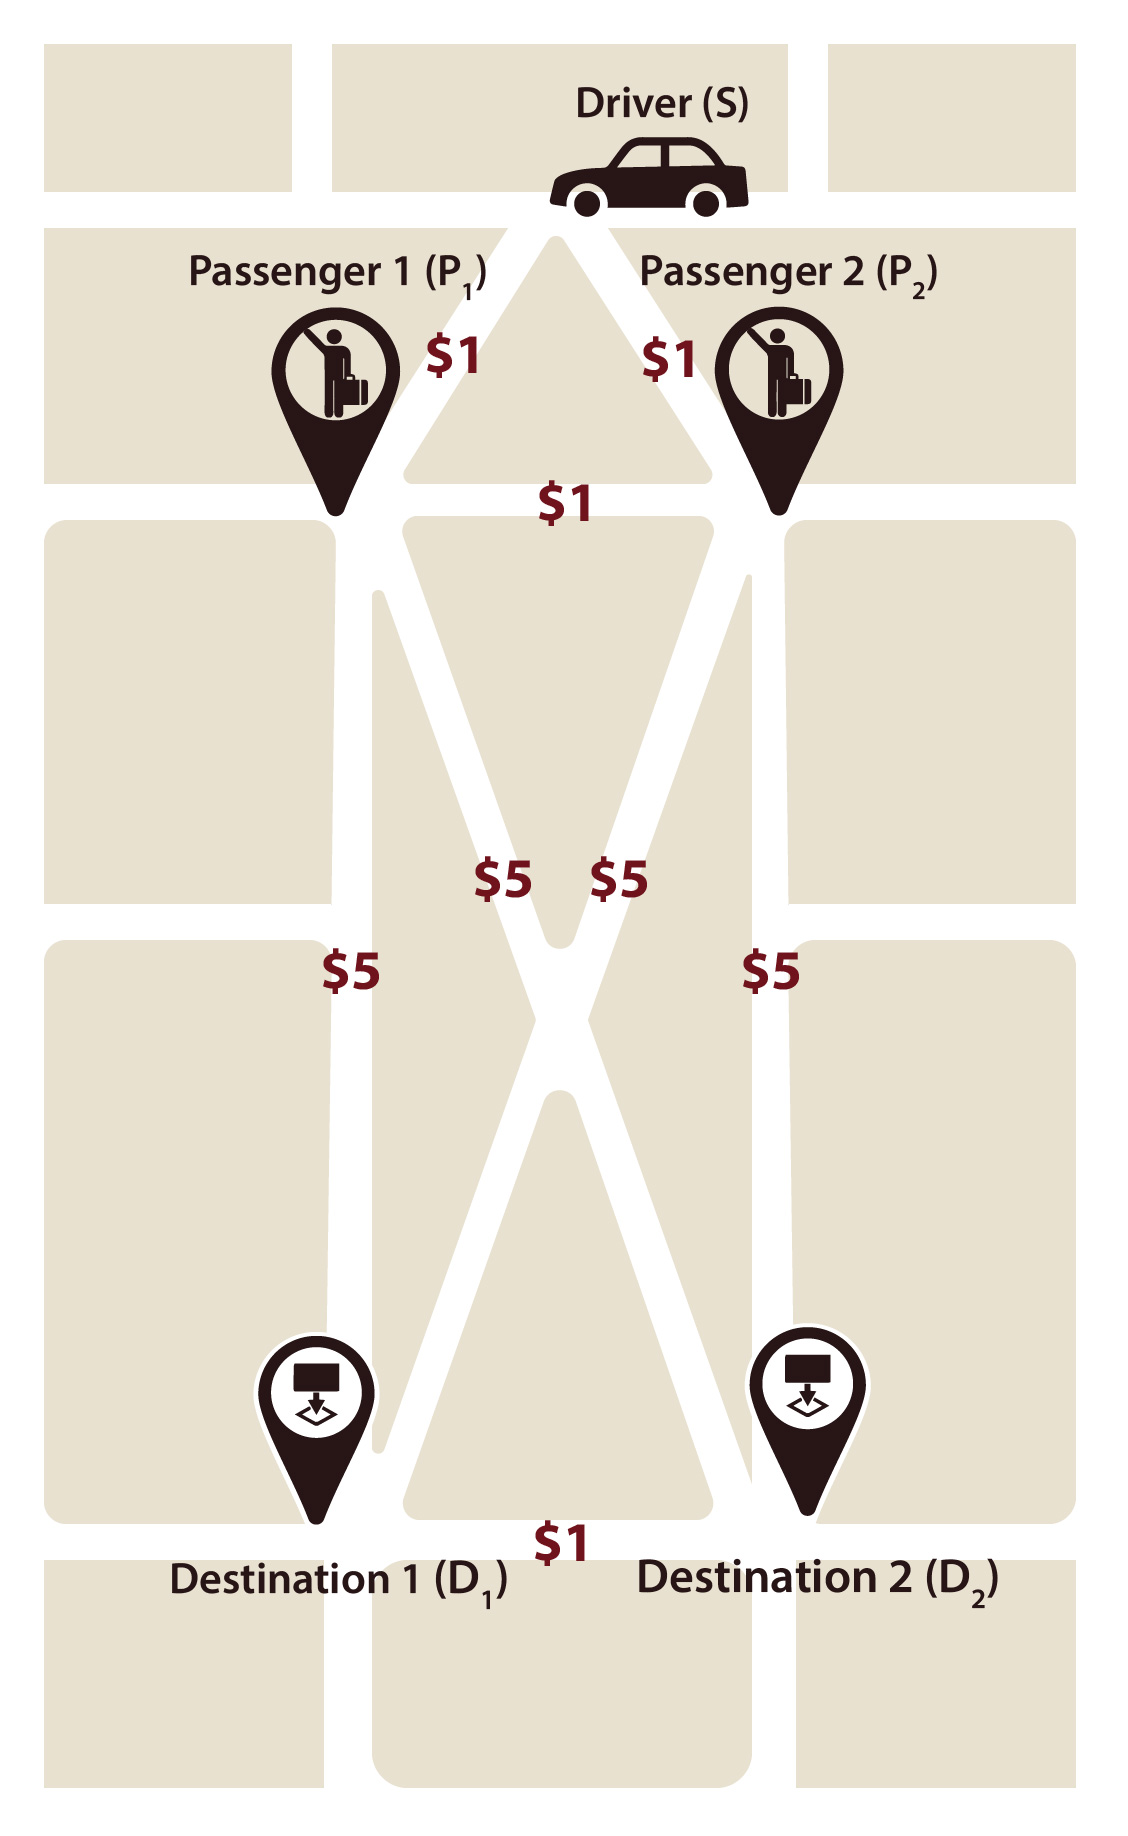
\includegraphics[width=6cm]{figures/mapV2.jpg}
  \caption{Example road network with driving fare and points of passengers and their destinations}
\end{figure}

\begin{figure}[htp]
  \centering
  \captionsetup{justification=centering}
  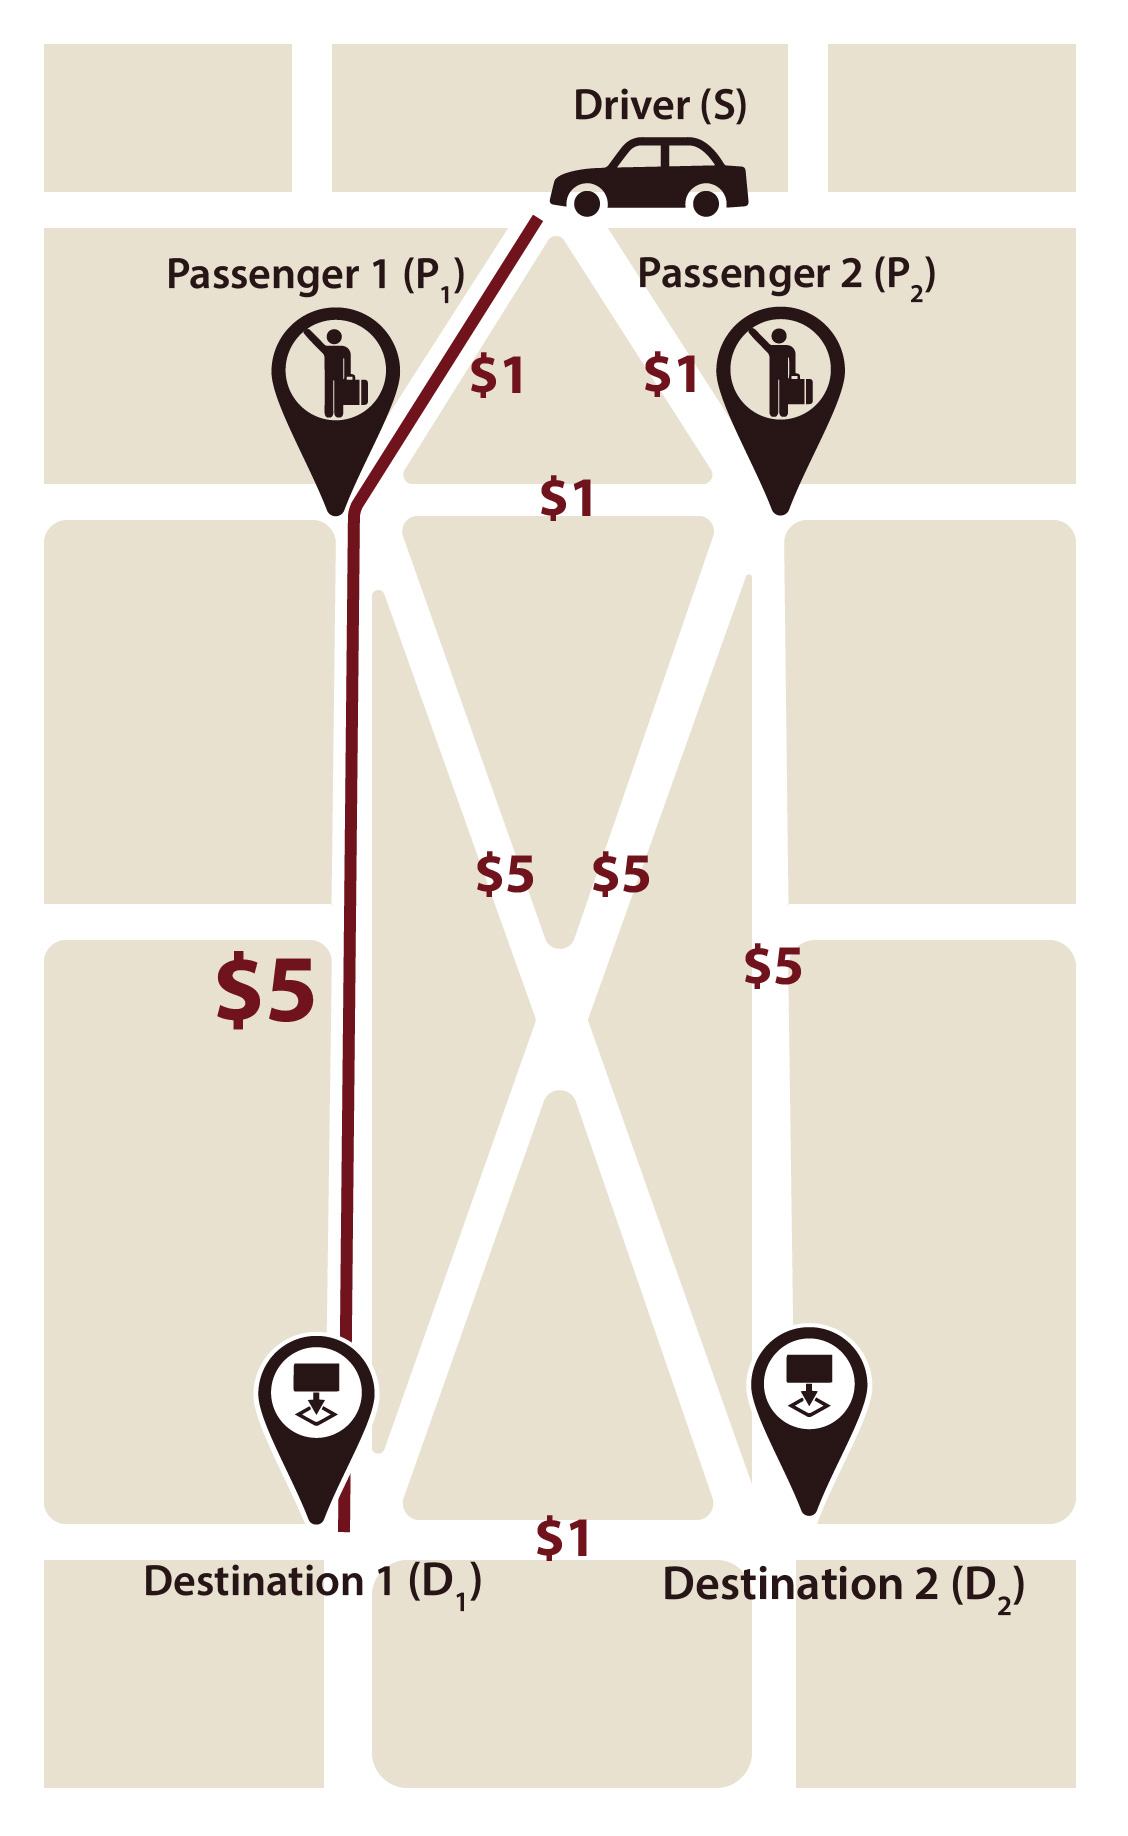
\includegraphics[width=6cm]{figures/mapV2_1.jpg}
  \caption{Best routing path when the driver only serving Passenger 1}
\end{figure}

\begin{figure}[htp]
  \centering
  \captionsetup{justification=centering}
  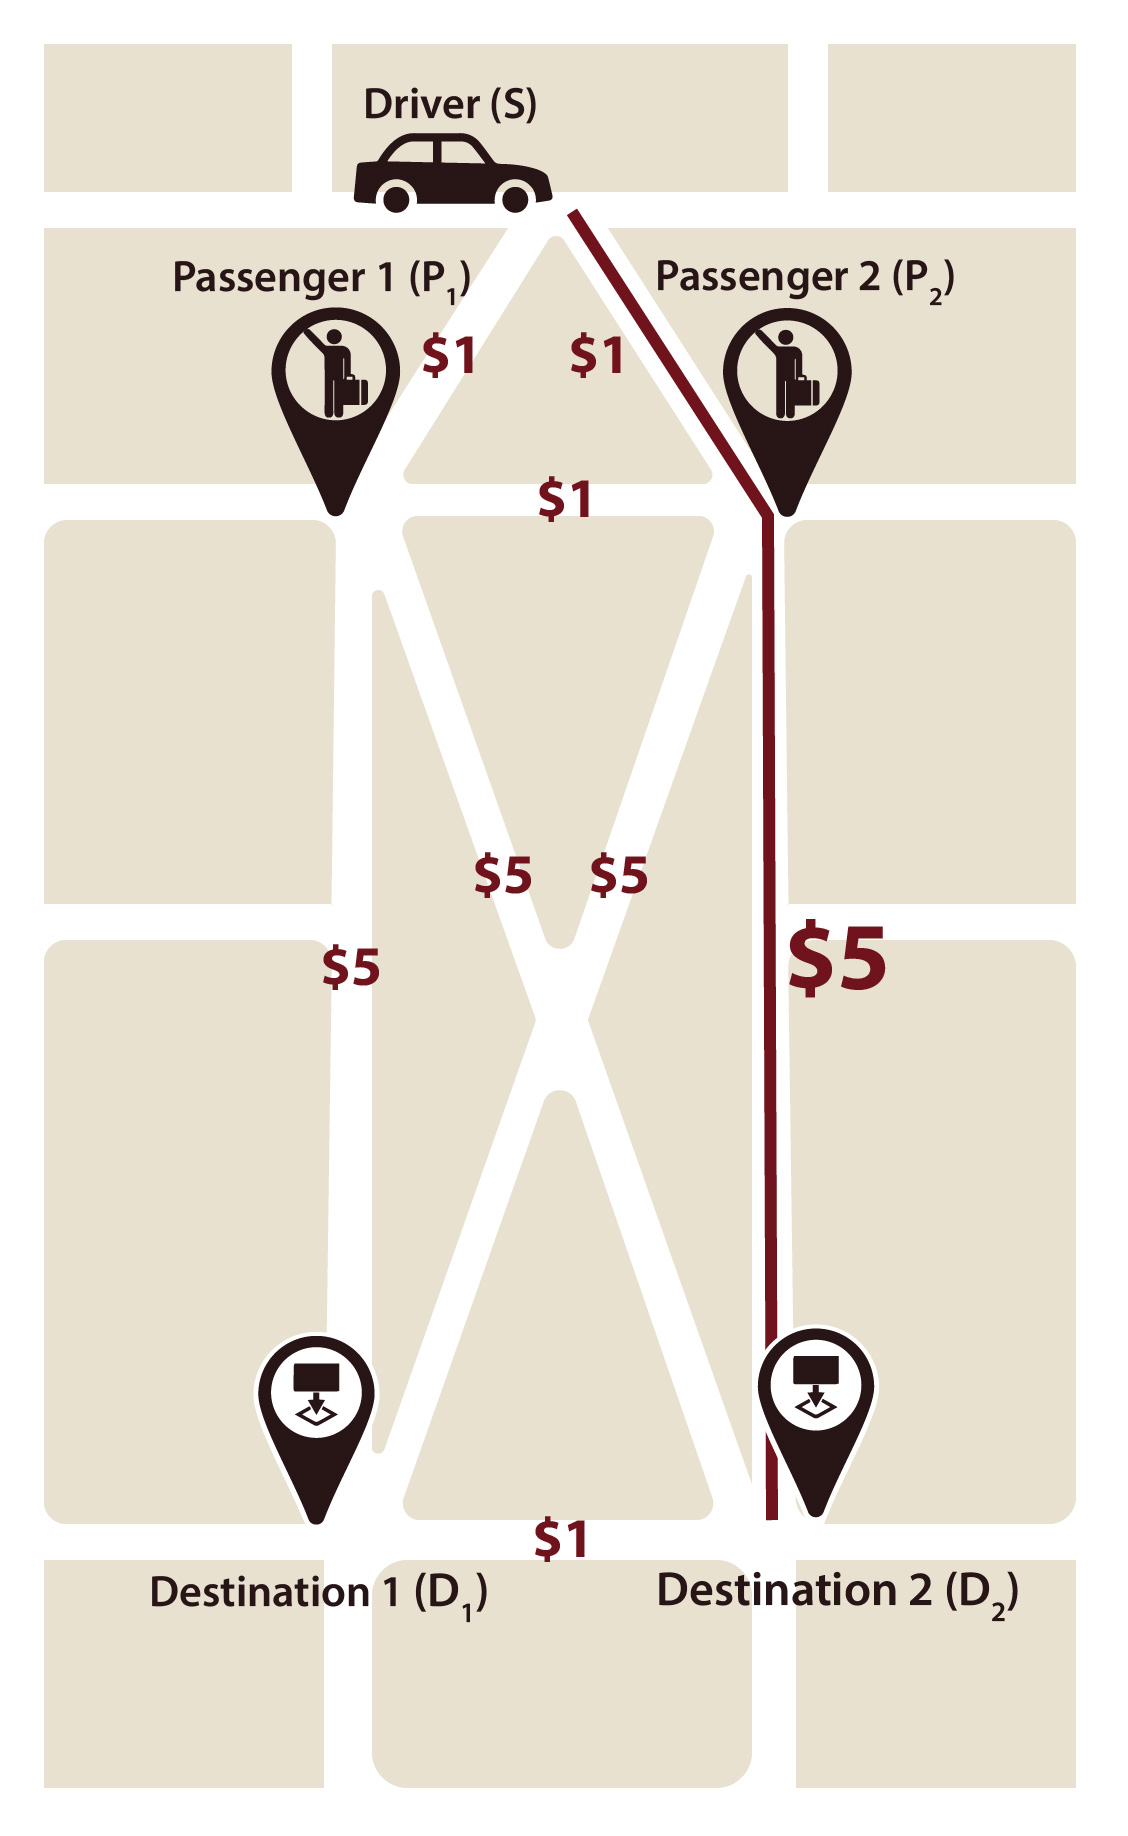
\includegraphics[width=6cm]{figures/mapV2_4.jpg}
  \caption{Best routing path when the driver only serving Passenger 2}
\end{figure}

\begin{figure}[htp]
  \centering
  \captionsetup{justification=centering}
  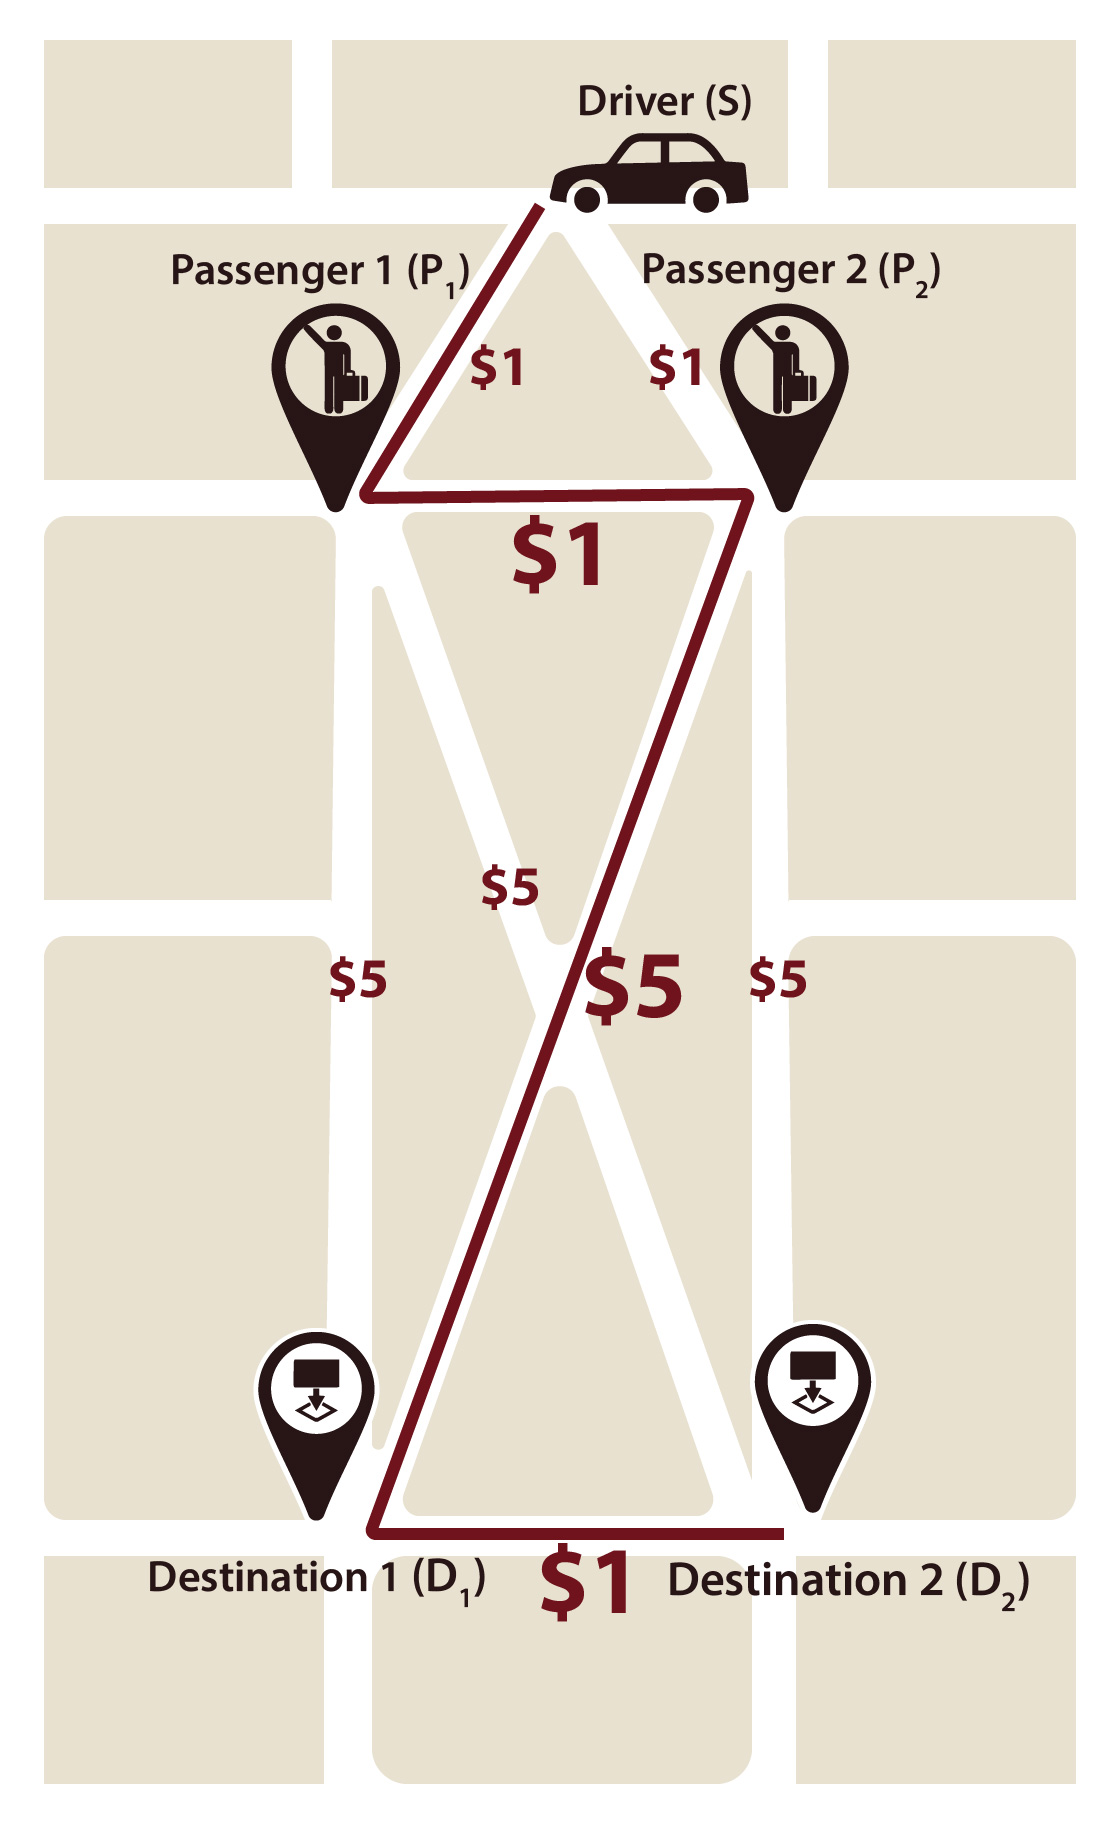
\includegraphics[width=6cm]{figures/mapV2_2.jpg}
  \caption{One of the best routing when both Passenger 1 and Passenger 2 carpool}
\end{figure}

\begin{figure}[htp]
  \centering
  \captionsetup{justification=centering}
  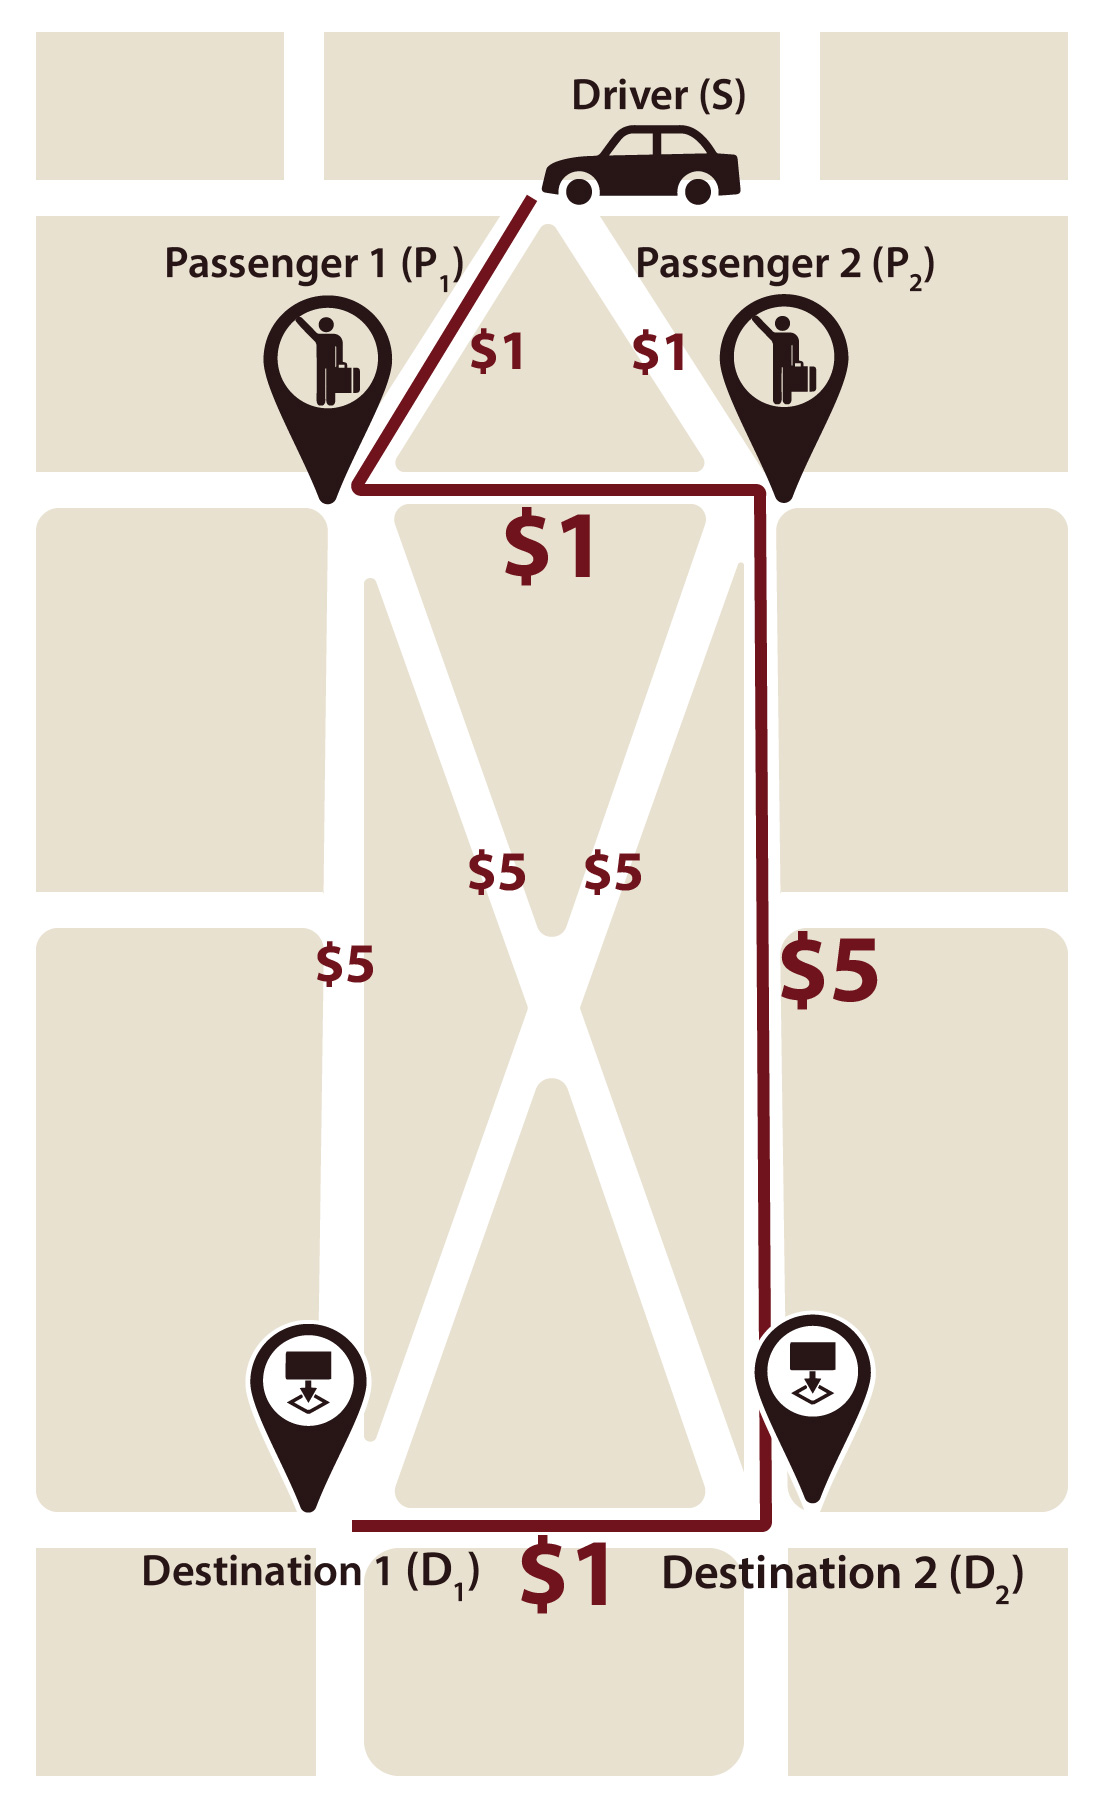
\includegraphics[width=6cm]{figures/mapV2_3.jpg}
  \caption{Another best routing when both Passenger 1 and Passenger 2 carpool}
\end{figure}
\newpage

\subsection{Fairness of Vehicle Dispatching}

In order to consider the fairness when dispatching driver, we introduce Jain's fairness index to avoid unfair situation:

$Firness\ Index = f_A(x) = \frac{\left(\sum\limits_{i=1}^{n} x_i\right)^2}{n \sum\limits_{i=1}^{n} x_i^2}$

We take accumulate driving requests that a driver has received as the metrics for fairness. That is, when a driver receives more driving requests in the past, he/she should give his/her chance of receiving a new driving request to the one who takes fewer driving requests.

As a new driving request comes, we need to ensure our system must get more or at least keep the same fairness. Hence, we form a constraint that the fairness index can not decrease compared to the previous fairness index.

However, when the driving resource changes, such as a new driver joins our system, it will violate our constraint for fairness. Because the newcomer has not taken any driving request before, the fairness will decrease. Even if a driver leaves our system, the fairness will increase or decrease due to the driver's situation. As a result, we need to reset the fairness index to the initial state and reset all the drivers' accumulated driving requests to 0. Nevertheless, it will make the fairness index's denominator to 0, which can not be divided. To avoid this situation, we assign a virtual driver with one accumulated driving request, which will make the fairness index to $\frac{1}{(n+1)}$, where $n$ is the number of drivers in our system. Moreover, for any situation that the fairness index will decrease when dispatching a new driving request, the fairness will reset.

\section{Mathematical Model}

\renewcommand\arraystretch{1.5}
\par
\begin{table}[ht]
  \centering
  \caption{Notations of given parameters}
  \begin{tabularx}{\textwidth}{cX}
  \toprule
  Notation & Description \\
  \midrule
    $R$ & Set of drivers in the system (take $i$ as index) \\
    $P$ & Set of passengers in the system (take $j$ as index) \\
    $D$ & Set of destinations in the system (take $k$ as index) \\
    $L$ & Set of links on the road network \\
    $P_r$ & Set of all paths for driver $r$, where $r \in R$ \\
    $B_r$ & Set of passengers that driver $r$ has picked up, where $r \in R$ \\
    $a_l$ & The fare for the link $l$, where $l \in L$ \\
    $Q_r$ & Maximum load capacity for driver $r$, where $r \in R$ \\
    $\delta_{pl}$ & Indicator function which is 1 if link $l$ on the route $r$ is selected; 0 otherwise \\
  \bottomrule
  \end{tabularx}
\end{table}  
\par

\begin{table}[ht]
  \centering
  \caption{Notations of decision variables}
  \begin{tabularx}{\textwidth}{cX}
  \toprule
  Notation & Description \\
  \midrule
  $x_p$ & Binary variable that indicates where route $p$ is chosen, $p \in P_z$. 1 if $p$ is chosen; 0 otherwise. \\
  $y_l$ & Binary variable that indicates whether link $l$ is on the shortest path. 1 if $l$ is on the shortest path; 0 otherwise. \\
  \bottomrule
  \end{tabularx}
\end{table}  
\newpage

\subsubsection*{Objective function}

\begin{align*}
  max\ min\ \frac{Original\ cost_i - carpool\ cost_i}{Original\ cost_i}
\end{align*}

\subsubsection*{Constraints}

\begin{align*}
  s.t. & \sum\limits_{p \in P_z} x_p = 1 && for\ v_i \ \& \ u_i, i \in \{1,2,...,n\} \tag{1} \\
  & \sum\limits_{p \in P_z} x_p \delta_{pl} = y_l && \forall l \in L \cup L' \cup L'' \tag{3} \\
  & y_l = 1 && \forall l \in L' \cup L"" \tag{4} \\
  & \sum\limits_{p \in P_w} z_p \delta_{pl} \leq y_l && \forall w \in V \cup U = W \tag{5} \\
  & \sum\limits_{p \in P_w} z_p = 1 && \forall w \in W \tag{6} \\
  & z_p = 0 \ or \ 1 \tag{7} \\
  & \sum\limits_{l \in L \cup L'} \sum\limits_{p \in Q_{v_i}} z_p \delta_{pl} a_l \leq \sum\limits_{l \in L \cup L'} \sum\limits_{p \in Q_{u_i}} z_p \delta_{pl} a_l && \forall i \in \{1,2,,...,n\} \tag{8} \\
\end{align*}
